% SPDX-License-Identifier: CC-BY-4.0
% Kshana arXiv preprint. Build: tectonic main.tex  (or pdflatex+bibtex x2)
\documentclass[11pt]{article}

\usepackage[utf8]{inputenc}
\usepackage[T1]{fontenc}
\usepackage{lmodern}
\usepackage[margin=1in]{geometry}
% Absorb the rare overfull line caused by unbreakable \texttt{} tokens
% (e.g. wasm-pack, satellite.js) without loosening normal paragraphs.
\setlength{\emergencystretch}{2em}
\usepackage{amsmath}
\usepackage{amssymb}
\usepackage{graphicx}
\usepackage{booktabs}
\usepackage{array}
\usepackage{siunitx}
\usepackage{xcolor}
\usepackage[colorlinks=true,linkcolor=black,citecolor=black,urlcolor=blue]{hyperref}
\usepackage[numbers,sort&compress]{natbib}
\usepackage{orcidlink}

\newcommand{\code}[1]{\texttt{#1}}
\graphicspath{{./}{../}{../crossover/}}

\title{\textbf{Kshana: An Open, Reproducible Engine for PNT-Resilience
Comparison, with a Quantum-versus-Classical Crossover Map under Parameter
Uncertainty}}

\author{Chakshu Baweja\,\orcidlink{0009-0008-2098-0751}\\
\small Ashforde O\"U, Estonia \\
\small \texttt{contact@ashforde.org}}

\date{\today}

\begin{document}
\maketitle

\begin{abstract}
Resilient positioning, navigation, and timing (PNT) underpins aviation,
defence, critical infrastructure, and emerging cislunar operations, yet the
field lacks a common basis for comparing how candidate resilience measures --
classical or quantum -- perform when GNSS is denied. Such comparisons are
predominantly private and non-reproducible: the authoritative recent survey of
quantum PNT names no open, reproducible tool for quantum-versus-classical
evaluation \citep{quantumpntreview2026}, and broader GNSS work has documented
how rarely reported results can be regenerated end to end
\citep{fernandezprades2018reproducibility}. We address this with a methodology
in which every result is reproducible from a committed scenario, random seed,
and engine version; every figure of merit carries an explicit
validated-or-not-modeled label; and the quantum/classical axis is a single
parameter swap inside one neutral code path, so the two are never compared
across separate implementations. The methodology is instantiated in Kshana
\citep{baweja2026kshana}, an open engine written in Rust with native, Python,
and WebAssembly targets and 19 scenario kinds. The new result is a Monte-Carlo
crossover/break-even map over the published-parameter envelope, with 95\%
bootstrap confidence intervals, identifying where a cold-atom inertial sensor or
optical-lattice clock changes the GNSS-outage outcome and where it does not.
Trust evidence is reported separately and tiered by strength: reference frames
agree bit-for-bit with SOFA/ERFA, SGP4 matches the AIAA 2006-6753 set to
\SI{4.12}{\milli\metre} worst-case, Allan deviations match NIST references, and
force-model validation by ephemeris fitting against agency precise ephemerides
yields a full-arc Galileo residual of \SI{0.61}{\metre} at degree/order 70.
Quantum-sensor figures are performance-model projections from cited device
literature, not measurements; the spoofing detector is characterised against
published TEXBAT parameters, not raw IQ.

\end{abstract}

\section{Introduction}\label{sec:intro}

Position, navigation, and timing (PNT) underpins power-grid synchronisation,
financial timestamping, telecommunications, and essentially every form of
autonomous and crewed mobility. In practice that infrastructure leans almost
entirely on global navigation satellite systems (GNSS), whose signals arrive at
the Earth's surface tens of decibels below the thermal noise floor and are
therefore trivially denied: low-cost jammers, meaconing, and increasingly
sophisticated spoofers can suppress or counterfeit a GNSS fix over a wide
area~\citep{misra2010,kaplan2017}. The operational consequence is loss of a
\emph{reference}, not merely of a gadget. The question that matters during an
outage is how long a platform can hold its position and time to within a stated
tolerance once the satellites can no longer be trusted. We refer to this
property as \emph{PNT resilience}: the growth of position and timing error
against outage (or holdover) duration, for a given on-board sensor suite.

A platform rides through a GNSS outage on whatever it carries. Inertial sensors
let it dead-reckon, but their error grows super-linearly as bias and
random-walk noise integrate twice into position~\citep{groves2013}; a local
clock holds time, but only until its own instability accumulates past the
allowed offset~\citep{riley2008nist}. The classical floor for both is well
characterised. The open question, and the subject of sustained investment, is
whether \emph{quantum sensing} meaningfully raises that floor. Cold-atom
interferometric accelerometers and gyroscopes promise bias stability and scale
factors set by atomic constants rather than by a drifting proof mass; optical
atomic clocks reach fractional frequency instabilities orders of magnitude below
chip-scale or even flight-qualified microwave standards; and optical two-way
time transfer offers a path to disseminate that stability between platforms.
The common thread is a \emph{slower error-growth law}: if the per-second noise
and the long-term drift are smaller, the error crosses any fixed tolerance later,
extending the survivable outage. Recent reviews survey this case in
detail~\citep{coldatomnavreview2022,quantumpntreview2026}. Tellingly, those same
reviews concede that quantitative comparisons across the field are difficult to
audit: they frequently rest on generic synthetic scenarios, mismatched figures
of merit, and proprietary trade studies whose assumptions are not published.
That concession matters, because it names the gap precisely: the resilience
debate is starved not of physics but of \emph{reproducible, falsifiable,
like-for-like comparison}.

The gap is real, and it is worth establishing by evidence. A number of capable
open tools exist, but each answers a different question and
none reproduces an end-to-end quantum-versus-classical resilience comparison on a
single neutral code path. RTKLIB~\citep{takasu2009} is a mature open package for
processing real GNSS observations into precise positions, but it concerns the
fix itself, not the post-outage error-growth dynamics of an inertial or clock
holdover. \texttt{gnss\_lib\_py}~\citep{knowles2024gnsslibpy} provides a clean
Python substrate for GNSS measurement analysis and algorithm prototyping, again
on the receiver-processing side rather than the resilience side. LuPNT
\citep{iiyama2023lupnt} targets lunar PNT architecture studies and is the
closest in scope to the multi-domain resilience question, yet it is an
architecture simulator, not an instrument for swapping a quantum sensor model
against its classical counterpart under controlled uncertainty. NaveGo
\citep{gonzalez2017navego} is a well-validated open inertial-navigation toolkit
with published error profiles (genuinely strong on the inertial axis), but it
models classical IMUs and does not carry clock-holdover, time-transfer, or
quantum-sensor models. None of these is unfalsifiable; the point is the
converse. Each is a sound tool for its own question, and the absence is the
\emph{intersection}. To our knowledge no open tool runs the full PNT resilience
stack of inertial dead-reckoning, clock holdover, and time transfer with a
quantum and a classical configuration exercised through the same code path,
seed-reproducibly, with uncertainty propagated.

This paper presents Kshana, an open engine built to close that intersection, and
uses it to produce a genuinely new result. The engine's external-validation
battery (Section~\ref{sec:validation}) establishes that its underlying
mechanics are trustworthy: frames bit-for-bit against SOFA/ERFA, SGP4 to
millimetre agreement against the AIAA reference set, Allan deviation against
NIST and Stable32, and force-model validation by ephemeris fitting against
agency precise orbits. That battery is \emph{evidence}, not the
contribution. The contribution is the reproducible crossover study built on top
of it (Section~\ref{sec:crossover}). Instead of reporting a single hero number,
we sweep each quantum lever across its published-parameter envelope by
Monte-Carlo and report the resilience advantage as a distribution with 95\%
confidence intervals, then locate the \emph{break-even} against the classical
baseline. The result is a map of \emph{when} quantum sensing changes the outcome
and when it does not. For the inertial lever, the cold-atom accelerometer's
advantage over a navigation-grade IMU is decisive at low platform vibration but
the break-even migrates toward higher vibration as the outage lengthens, so the
honest answer is conditional on the host platform's mechanical environment. For
the clock lever, an optical-lattice standard and a flight-qualified maser hold
sub-microsecond time across a full 24~h holdover in our envelope, whereas a
deployed chip-scale clock crosses the same threshold near eight and a half
hours: a same-maturity comparison that separates what is demonstrated in the
lab from what flies today. We label every quantum result as a performance-model
projection, not a measurement, and carry its technology-readiness tag inline.

We claim no superiority on any single axis, and we use ``to our knowledge, no
open tool \ldots'' rather than ``first'' or ``only.'' In-browser orbit
propagation, for instance, is not new~\citep{satellitejs}; our delta is that a
single engine runs the full integrated stack zero-install. With that framing,
our contributions are:

\begin{enumerate}
  \item \textbf{A reproducible quantum-versus-classical resilience crossover map
  under parameter uncertainty} (the new result, Section~\ref{sec:crossover}).
  For each quantum lever (cold-atom inertial, optical-lattice clock, optical
  time transfer), a Monte-Carlo sweep over the published-parameter envelope
  yields the resilience-figure-of-merit advantage as a distribution with 95\%
  confidence intervals and identifies the break-even against the classical
  baseline, answering \emph{when} quantum sensing changes the outage outcome,
  openly and from a committed scenario and seed.

  \item \textbf{A reproducibility-and-falsifiability methodology} for
  resilient-PNT comparison (Section~\ref{sec:method}): a scenario-plus-seed-plus-
  version reproducibility triple, a per-figure-of-merit \emph{validated} or
  \emph{not-modeled} label, and hand-derived oracle tests. It builds on prior
  reproducible-research practice~\citep{fernandezprades2018reproducibility,nasastd7009};
  the genuinely new element is the requirement that the quantum and classical
  configurations differ only by a parameter swap on a \emph{single neutral code
  path}, so that any reported advantage is attributable to the device model and
  not to two divergent implementations.

  \item \textbf{One open engine instantiating the methodology across the PNT
  stack} (Section~\ref{sec:arch}): a Rust core with native, Python, and
  WebAssembly targets, 19 scenario kinds, and standard-format interoperability
  (RINEX, SP3, CCSDS OEM/OMM), summarised with its capabilities \emph{and}
  non-capabilities stated symmetrically in Table~\ref{tab:intersection}.

  \item \textbf{An external-validation battery, tiered by strength}
  (Section~\ref{sec:validation}, Table~\ref{tab:validation}): bit-for-bit checks
  against authoritative oracles (frames, SGP4, Allan deviation); post-fit
  residuals against real agency precise ephemerides, with the force-model-fit,
  arc-length, and gravity-degree caveats stated inline (full-arc Galileo
  $0.61$~m at degree/order~70 as the headline; the reduced-dynamic
  empirical-acceleration tier reported as a labelled bound, not a measurement of
  force-model accuracy; LRO $6.6$~m, above the $5$~m target, stated honestly);
  and a controlled, reproducible cross-validation showing the kernel-free
  analytic stack reproduces a DE440/ANISE realisation for the LRO reduced-dynamic
  arc, consistent with established results~\citep{bertone2021grail,li2023leopod}
  and presented as a reproduction scoped to that arc, not a discovery.

  \item \textbf{A multi-layer spoofing detector}, characterised against published
  TEXBAT \emph{parameters} (Section~\ref{sec:validation}), with raw-IQ ingestion
  stated as future work; it sits explicitly in the not-externally-validated tier.
\end{enumerate}

The remainder of the paper develops the methodology that makes these claims
falsifiable (Section~\ref{sec:method}), situates the engine against related open
tools (Section~\ref{sec:related}), summarises its architecture
(Section~\ref{sec:arch}), presents the crossover study
(Section~\ref{sec:crossover}) and the tiered validation
(Section~\ref{sec:validation}), and states the limitations and threats to
validity (Section~\ref{sec:limitations}), chief among them that the
quantum-sensor figures throughout are model projections from cited device
literature, not measurements.

\section{A methodology for credible PNT-resilience comparison}\label{sec:method}

The difficulty in comparing resilient-PNT technologies is rarely the physics; it
is establishing that two reported numbers were produced under conditions
comparable enough to be set against each other. A claimed advantage for a
quantum sensor over a classical one may reflect the sensor, or it may reflect a
different propagator, a different error model, an unstated parameter choice, or
simply a different random seed. We therefore treat the comparison protocol
itself as the object of design, and require any quantitative claim emitted by
the engine to satisfy a three-part contract. The contract is not a code-quality
aspiration; each clause is mechanically enforced, and a result that violates any
clause is not reported.

\paragraph{(a) Reproducible from scenario, seed, and engine version.}
Every figure of merit is a deterministic function of a committed scenario
specification, an explicit pseudo-random seed, and a pinned engine version.
Given those three inputs the engine produces \emph{bit-identical} output: floating-point
results are reproduced exactly across re-runs on the same target, not merely to
within a tolerance. Determinism is a property of the implementation
(seeded generators threaded explicitly, no wall-clock or
unordered-iteration dependence in the numerical path), so a third party can
regenerate any reported value from the artifacts alone. This makes a claim
\emph{auditable}: a referee who disputes a number reruns the named scenario at
the named seed and version and obtains the same bits, or finds that they do not.
The exact commands to regenerate every figure and headline number in this paper
are listed in the reproducibility appendix.

\paragraph{(b) Every figure of merit is labelled validated or not-modeled.}
We attach to each reported quantity a machine-checkable status drawn from a
fixed vocabulary: \emph{validated} (the quantity is anchored to an external
oracle or a real reference dataset, with the anchor named), or \emph{not-modeled}
(the quantity is a model projection with no external anchor, and the absence of
an anchor is declared). The status is carried alongside the number rather than
left to prose, so the validation tier of any figure of merit is recoverable
without trusting the narrative. This discipline is what keeps the
trust evidence (Section~\ref{sec:validation}, Table~\ref{tab:validation})
honestly separated from the projections: a frames check against SOFA/ERFA and a
cold-atom-IMU dead-reckoning curve are both numbers the engine emits, but only
the first is externally anchored, and the label says so. In particular, the
quantum-sensor figures throughout this paper are performance-model projections
from cited device coefficients, not measurements; they carry the not-modeled
label and a technology-readiness tag wherever they appear
(Section~\ref{sec:crossover}).

\paragraph{(c) The quantum-versus-classical axis is a single neutral code path.}
The comparison that is the subject of Section~\ref{sec:crossover} is performed by
\emph{the same code} evaluated with different published coefficients, not by two
separate implementations. A cold-atom accelerometer and a navigation-grade IMU
are driven through one dead-reckoning path; an optical-lattice clock and a
chip-scale atomic clock through one holdover path. Only the device coefficients
differ, sourced from the respective device literature. The consequence is that
any difference in the resulting figure of merit is attributable to the sensor
parameters, not to two divergent code paths that might differ in integration
scheme, error accounting, or numerical conditioning. This removes the most
common confound in cross-technology PNT comparison, in which the quantum and
classical estimates come from different tools and the gap cannot be cleanly
ascribed.

\paragraph{Falsifiability via hand-derived tests.}
The three clauses make results reproducible and honestly labelled, but
reproducibility alone does not establish correctness: an engine can deterministically
reproduce a wrong number. We therefore require that the expected
value in every test be derived by hand from physics or from an external
reference, never read back from the engine. Frame-rotation expectations come
from closed-form rotations and the SOFA/ERFA reference values; clock-stability
expectations from analytic Allan-variance relations and NIST/Stable32 reference
data; geometric-dilution expectations from the closed-form GDOP. Because the
oracle is independent of the implementation, a regression that silently changes a
result is caught: the engine is falsifiable against an external standard rather
than self-consistent with its own prior output.

\paragraph{What is new relative to prior reproducible-research work.}
Reproducibility and model-credibility frameworks for this domain exist, and we
build on them. \citet{fernandezprades2018reproducibility} establish continuous
reproducibility for GNSS signal processing, but their scope is the raw-IF
receiver chain; the resilient-PNT figures of merit considered here (inertial
dead reckoning, clock holdover, time-transfer budgets, orbit residuals) lie
outside it. \citet{nasastd7009} provide a thorough modelling-and-simulation
credibility regime, but it is a heavyweight governance process intended for
agency programs, not a lightweight protocol a single open tool can enforce on
every emitted number. To our knowledge, no open tool combines, across the full
resilient-PNT stack, the two elements we treat as load-bearing: the
\emph{single-code-path parameter swap} as the required mechanism for any
quantum-versus-classical comparison, and the \emph{per-figure-of-merit,
machine-checkable validated/not-modeled label} carried with each result. Those
two requirements, applied together across the stack, are what is new here; the
engine of Section~\ref{sec:arch} is one instantiation of them.

\section{Background and the capability landscape}\label{sec:related}

The resilient-PNT comparison problem sits at the confluence of three well-developed
but separate tool ecosystems. Kshana does not displace any of them; it occupies the
intersection they leave open. We organise the landscape into three honest tiers and
make the boundaries explicit in Table~\ref{tab:intersection}.

\paragraph{Tier 1: quantum-navigation simulations.}
A growing body of work simulates quantum inertial and timing sensors, but almost
always from a quantum-specific, fusion-or-enhancement standpoint rather than as a
neutral quantum-versus-classical comparison harness. Atom-interferometric strapdown
navigation has been simulated end-to-end with a cold-atom accelerometer in the loop
\citep{atomstrapdown2023}, and high-fidelity simulators model the cold-atom
interferometer (CAI) at the level of fringe contrast and projection noise
\citep{quantumnav2025highfidelity}. We concede that the latter achieves
\emph{higher} fidelity than Kshana on the single inertial lever: its first-principles
CAI model is more detailed than our coefficient-driven projection. Hybrid
cold-atom/classical inertial estimation has likewise been demonstrated in an EKF
framework that fuses a CAI with a conventional IMU \citep{hybridcai2018}. These are
quantum-axis simulators; none provides a single neutral code path in which the same
scenario is run with a quantum or a classical sensor and the resilience figure of
merit compared like for like. The closest quantum-versus-classical service we are
aware of, TNO SENSED \citep{tno_sensed}, is closed and not reproducible: its
parameters, seeds and code are not publicly available, so its comparisons cannot be
independently re-derived. The field's own reviews note the absence of an open,
reproducible quantum-versus-classical comparison capability
\citep{coldatomnavreview2022,quantumpntreview2026}; in particular,
\citet{quantumpntreview2026} names no open reproducible quantum-versus-classical
PNT tool.

\paragraph{Tier 2: open navigation frameworks.}
Open, citable navigation frameworks already embody parts of the methodology we build
on. NaveGo \citep{gonzalez2017navego} establishes the interchangeable-error-model
pattern for inertial navigation -- a sensor is described by a parameter profile and
swapped without touching the estimator -- and we reuse its validated navigation-grade
IMU profiles as the classical baseline for the inertial lever. It has, however, no
quantum axis. Among open PNT and GNSS tools, LuPNT \citep{iiyama2023lupnt} is an
excellent, well-engineered library for lunar positioning, and gnss\_lib\_py
\citep{knowles2024gnsslibpy} is a similarly strong toolkit for real-data GNSS
analysis. We differentiate from these on the axes they do not target -- a
single-code-path quantum-versus-classical swap, and the reproducibility-triple
methodology (Section~\ref{sec:method}) -- and explicitly \emph{not} on engineering
quality, which in both cases is high. LuPNT is lunar-scoped; gnss\_lib\_py is oriented
to processing real observations rather than forward performance simulation.

\paragraph{Tier 3: astrodynamics and real-signal tools.}
The astrodynamics and real-signal ecosystem answers a fundamentally different
question. RTKLIB and comparable GNSS engines \citep{takasu2009} post-process real
pseudorange and carrier-phase observations to produce a position fix; GMAT
\citep{nasa_gmat} and Orekit \citep{orekit} are high-fidelity mission-design and
orbit-determination frameworks; the \code{sgp4} crate \citep{sgp4crate} is a
production analytic propagator; and Nyx with ANISE \citep{nyxanise} provides
DE-ephemeris-grade dynamics and serves in this work as a reference oracle, not a
rival. These tools consume real signals or drive high-fidelity mission analysis.
Kshana is the upstream \emph{forward performance simulator}: it asks, for a given
scenario, seed and sensor parameterisation, how a resilience figure of merit behaves,
before any real observation exists. In-browser SGP4 propagation is itself not new
\citep{satellitejs}; the delta here is a single engine running the full integrated
stack zero-install in WebAssembly, not the propagator alone.

To our knowledge, no open tool combines a single-code-path quantum-versus-classical
swap, seed-level reproducibility, and a terrestrial-plus-lunar resilience scope in one
deployable engine. Table~\ref{tab:intersection} states this symmetrically, listing the
axes Kshana lacks alongside those it has.

\begin{table}[t]
\centering
\small
\setlength{\tabcolsep}{4pt}
\caption{Capability landscape across representative tools. Columns include axes that
Kshana lacks (real-observation processing, PVT position fix, three-axis INS
mechanisation, raw-IQ spoofing) alongside axes it provides (single-code-path
quantum/classical swap, seed-level reproducibility, terrestrial-plus-lunar resilience
scope) and a deployment row. A checkmark ($\checkmark$) denotes a supported capability
and a dash (--) its absence. Kshana and RTKLIB answer different questions: RTKLIB
post-processes real signals into a position fix, whereas Kshana is an upstream forward
performance simulator. The comparison is one of scope, not quality.}
\label{tab:intersection}
\resizebox{\textwidth}{!}{%
\begin{tabular}{l c c c c c c c}
\toprule
& \rotatebox{90}{Quantum/classical}
& \rotatebox{90}{Seed-reproducible}
& \rotatebox{90}{Terr.+lunar resil.}
& \rotatebox{90}{Real-obs.\ proc.}
& \rotatebox{90}{PVT fix}
& \rotatebox{90}{3-axis INS mech.}
& \rotatebox{90}{Raw-IQ spoofing} \\
\midrule
Kshana \citep{baweja2026kshana}      & $\checkmark$ & $\checkmark$ & $\checkmark$ & --           & --           & --           & --           \\
LuPNT \citep{iiyama2023lupnt}        & --           & $\checkmark$ & --           & $\checkmark$ & $\checkmark$ & --           & --           \\
gnss\_lib\_py \citep{knowles2024gnsslibpy} & --     & $\checkmark$ & --           & $\checkmark$ & $\checkmark$ & --           & --           \\
NaveGo \citep{gonzalez2017navego}    & --           & $\checkmark$ & --           & --           & --           & $\checkmark$ & --           \\
RTKLIB \citep{takasu2009}            & --           & --           & --           & $\checkmark$ & $\checkmark$ & --           & --           \\
GMAT / Orekit \citep{nasa_gmat,orekit} & --         & --           & --           & $\checkmark$ & --           & --           & --           \\
TNO SENSED \citep{tno_sensed}        & $\checkmark$ & --           & --           & --           & --           & $\checkmark$ & --           \\
\code{sgp4} crate \citep{sgp4crate}  & --           & $\checkmark$ & --           & --           & --           & --           & --           \\
\bottomrule
\end{tabular}%
}

\vspace{0.4em}
{\small\emph{Deployment:} Kshana ships as a zero-install WebAssembly integrated
stack (the full pipeline in one engine), not as a single in-browser propagator.}
\end{table}

\section{Engine architecture}\label{sec:arch}

This section summarises the engine; it is the substrate for the methodology of
\S\ref{sec:method} and the crossover study of \S\ref{sec:crossover}, not a
contribution in itself. Breadth is stated and cited rather than treated in depth, to
keep the paper's load on the methodology and the new result.

Kshana \citep{baweja2026kshana} is a single Rust core driven by a small TOML scenario.
A scenario's \code{kind} field is resolved to a typed variant and the dispatcher
matches it exhaustively, so the catalogue of packs is compile-checked rather than
string-dispatched; an absent or unrecognised kind falls back to the historical clock
pack. The nineteen scenario kinds (eighteen named kinds plus the clock pack as the
historical default, in v0.16.0) span the resilient-PNT stack: clock holdover,
inertial dead-reckoning, terrestrial and lunar integrity (snapshot/solution-separation
Advanced Receiver Autonomous Integrity Monitoring, ARAIM, with protection levels),
two-way time transfer, hybrid and fusion estimation,
GNSS-INS coupling, GNSS signal simulation, jamming, spoofing and spoof detection,
ephemeris/ground-track propagation, gravity-map, terrain-aided, and combined alternative-PNT
navigation, and the one- and $N$-dimensional parameter sweeps (\code{sweep},
\code{sweep-nd}) that drive the Monte-Carlo crossover machinery of \S\ref{sec:crossover}.

Sensor and environment behaviours are independent modules. Each carries a published
\emph{provenance string} naming the device or reference whose coefficients it
instantiates---for example, the clock curves are tagged with the optical-lattice,
hydrogen-maser and chip-scale-atomic-clock sources and a maturity (TRL) label they were
parameterised from---so that every reported figure is traceable to its literature
source and its model-versus-measurement status is legible at the point of use. The run
harness composes the selected modules on a common timeline and emits a
schema-versioned, self-describing JSON record (engine version, scenario, and per-module
provenance carried inline) alongside an SVG chart that is stamped centrally with the
same identifying footer, so a saved figure or result file stands alone. This is the
machine-explicit ``validated-or-not-modeled per figure-of-merit'' contract of
\S\ref{sec:method} realised in the output format itself.

The same core compiles to three targets from one source tree, without a separate
re-implementation per platform: a native binary and library (the \code{rlib}/CLI used
for the validation battery of \S\ref{sec:validation}); a PyO3 extension module for use
from Python and notebooks; and a WebAssembly module (built with \code{wasm-pack}) that
runs the full integrated stack in the browser with zero install. In-browser orbital
propagation is not itself new---\code{satellite.js} \citep{satellitejs} has long
provided in-browser SGP4---so the contribution here is not the browser target but that
a \emph{single} engine, identical to the validated native build, runs the whole
integrated PNT-resilience stack client-side, which is what makes the reproducibility
contract of \S\ref{sec:method} portable to a reader with no toolchain.

For interoperability with established tooling the engine reads and writes
standard exchange formats: RINEX navigation and observation records, IGS SP3 precise
ephemerides, and the CCSDS Orbit Ephemeris and Orbit Mean-elements Messages (OEM/OMM).
These are the on-ramps and off-ramps to the agency and reference datasets used in
\S\ref{sec:validation}; the engine's scope and its non-capabilities (no
real-observation PVT, no full INS mechanisation, no raw-IQ ingestion) are stated
symmetrically in Table~\ref{tab:intersection}.

\section{A quantum-versus-classical resilience crossover map}\label{sec:crossover}

The contribution of this paper is not another single-point claim that a quantum
sensor outperforms its classical counterpart. It is a \emph{map}: for each
quantum lever, a grid of operating points across the realistic published-parameter
envelope, at every node of which we report the resilience figure of merit as a
distribution rather than a number, and against which we locate the
\emph{break-even} where the quantum advantage disappears. The question the map
answers is the one the field's own reviews say is open
\citep{quantumpntreview2026}: not \emph{whether} a cold-atom inertial sensor or an
optical clock can help during a GNSS outage, but \emph{when} --- under what outage
duration, platform environment, and device maturity --- it actually changes the
outcome, and when a same-maturity classical unit is the better choice.

Every result in this section is produced by the same machinery the validated packs
use. For each lever we sweep the operating grid with \code{nd\_sweep\_ensemble};
each node is a Monte-Carlo ensemble (64 seeds for the inertial study, 32 for the
clock) over the parameter envelope, and the figure of merit is summarised by its
mean, percentiles, and a 95\% bootstrap confidence interval computed by the same
bootstrap the ensemble packs apply elsewhere. The quantum and classical legs share
one neutral code path, swapped by parameters alone, so the comparison is never made
across two implementations. No new physics is introduced. The cold-atom noise is a
first-principles interferometer model --- a shot-noise term $1/(C\sqrt{N})$ in atom
number $N$ and contrast $C$, combined in quadrature with a platform-vibration floor
$\sqrt{S_a/(3T)}$ in the acceleration PSD $S_a$ and interrogation time $T$ --- and
the classical leg uses the NaveGo-validated inertial error profile
\citep{gonzalez2017navego}. We restate the binding caveat of
Section~\ref{sec:limitations} once here and rely on it throughout: \textbf{every
quantum figure in this section is a performance-model projection from
laboratory-maturity device coefficients, not a measurement.}

\subsection{Inertial: cold-atom versus navigation-grade dead reckoning}

The inertial lever pits a cold-atom accelerometer of the Exail/Templier class
\citep{templier2022} against a navigation-grade strapdown unit
\citep{groves2013}, both dead-reckoning position through a GNSS outage. We sweep
two axes that dominate the outcome: outage duration, from \SI{30}{\second} to
\SI{1800}{\second}, and the platform-vibration acceleration PSD, from
$1~\mu\mathrm{g}/\sqrt{\mathrm{Hz}}$ (an isolated, quiescent platform) to roughly
$3~\mathrm{mg}/\sqrt{\mathrm{Hz}}$ (a noisy host). The figure of merit is the
95th-percentile horizontal position error over the ensemble; the advantage at a
node is the classical 95th-percentile error divided by the quantum one.
Figure~\ref{fig:inertial} shows the full map.

\begin{figure}[t]
  \centering
  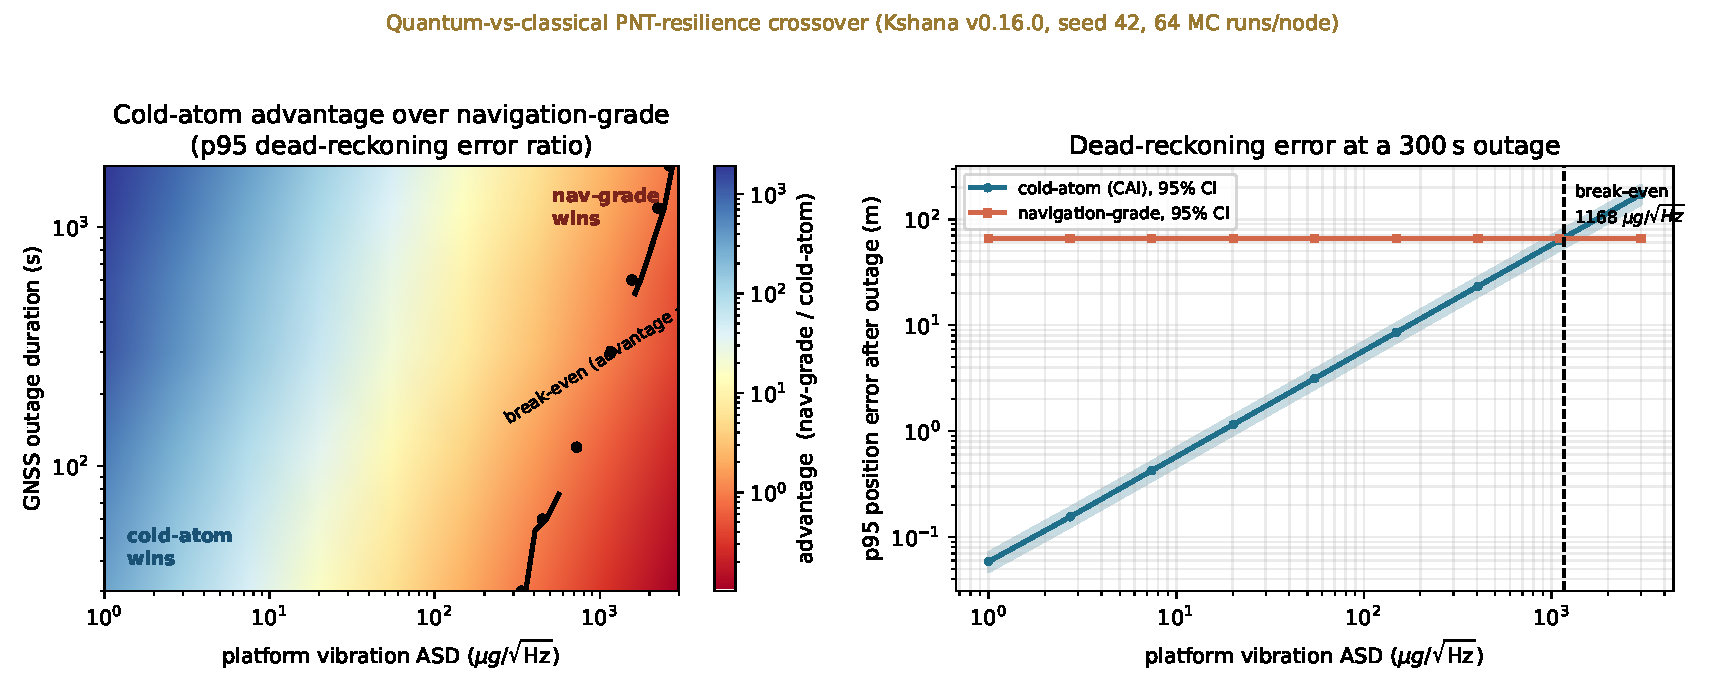
\includegraphics[width=0.95\linewidth]{inertial.pdf}
  \caption{Inertial crossover map. Cold-atom accelerometer (Exail/Templier class,
  \citealp{templier2022}) versus navigation-grade strapdown
  (\citealp{groves2013}), dead-reckoning 95th-percentile position error as a
  function of outage duration and platform-vibration acceleration PSD. Each node is
  a 64-seed Monte-Carlo ensemble with a 95\% bootstrap confidence interval; the
  dashed contour is the break-even (advantage~$=1$) where the navigation-grade unit
  matches the cold-atom sensor. The advantage is overwhelming on a quiet platform
  and erodes with vibration; the break-even PSD rises with outage duration. The
  quantum leg is a performance-model projection from laboratory-maturity device
  coefficients, not a measurement.}
  \label{fig:inertial}
\end{figure}

The first finding is that on an isolated platform the cold-atom advantage is large
and grows with outage length. At $1~\mu\mathrm{g}/\sqrt{\mathrm{Hz}}$ the advantage
is a factor of $307$ for a \SI{30}{\second} outage (cold-atom
\SI{2.5}{\milli\meter} versus navigation-grade \SI{0.75}{\meter} at the 95th
percentile), rising to $439$ at \SI{60}{\second} and to $1915$ at
\SI{1800}{\second}, where the navigation-grade error has grown to
\SI{2.3}{\kilo\meter} while the cold-atom error is near \SI{1.2}{\meter}. The
confidence intervals are tight relative to this gap --- the cold-atom 95th
percentile at the \SI{30}{\second}, $1~\mu\mathrm{g}/\sqrt{\mathrm{Hz}}$ node has a
bootstrap interval of $[2.0,\,2.9]~\si{\milli\meter}$ --- so the advantage on a
quiet platform is not a sampling artefact.

The second finding is that this advantage is conditional, and the map shows exactly
where it fails. As the vibration PSD rises the cold-atom error grows steeply, driven
by the $\sqrt{S_a/(3T)}$ vibration floor, while the navigation-grade error is
comparatively insensitive to it. The two curves cross: for a short
\SI{30}{\second} outage at a vibration level of
$\approx 405~\mu\mathrm{g}/\sqrt{\mathrm{Hz}}$ (about $0.4~\mathrm{mg}/\sqrt{\mathrm{Hz}}$)
the advantage falls to $0.75$ --- below unity, meaning the navigation-grade unit
\emph{wins}. On a vibrating host during a brief outage, the classical sensor is the
better choice, and the map says so plainly rather than reporting only the favourable
corner.

The third finding ties the first two together: the break-even vibration level rises
\emph{monotonically} with outage duration, from
$334~\mu\mathrm{g}/\sqrt{\mathrm{Hz}}$ at \SI{30}{\second} to
$2640~\mu\mathrm{g}/\sqrt{\mathrm{Hz}}$ at \SI{1800}{\second} (Table~\ref{tab:breakeven}).
The longer the outage, the more vibration the cold-atom sensor can tolerate before
losing. The mechanism is in the model: the cold-atom advantage over the
navigation-grade unit is dominated by the latter's accumulating bias error, which
grows roughly as $t^2$, whereas the cold-atom sensor's own vibration-limited error
is a random walk growing roughly as $t^{1.5}$. The bias term outruns the random-walk
term, so the duration at which the quantum sensor pays off increases the more
vibration it must endure --- the longer the outage, the wider the environmental
window in which it is the right tool.

\begin{table}[t]
  \centering
  \caption{Break-even platform-vibration PSD at which the navigation-grade unit
  matches the cold-atom sensor, as a function of outage duration. The break-even
  rises monotonically: a longer outage tolerates more vibration before the quantum
  advantage is lost.}
  \label{tab:breakeven}
  \begin{tabular}{rr}
    \toprule
    Outage duration (s) & Break-even PSD ($\mu\mathrm{g}/\sqrt{\mathrm{Hz}}$) \\
    \midrule
    30   & 334  \\
    60   & 448  \\
    120  & 724  \\
    300  & 1168 \\
    600  & 1565 \\
    1200 & 2250 \\
    1800 & 2640 \\
    \bottomrule
  \end{tabular}
\end{table}

\subsection{Clock: a same-maturity holdover ladder}

The clock lever asks how long each of three clock technologies can hold timing to a
\SI{1}{\micro\second} budget after its disciplining GNSS reference is lost. We
deliberately frame this as a technology-readiness ladder rather than a single
contest, because the three rungs are not the same maturity and a like-for-like
winner-flip does not exist here: a ground-laboratory strontium optical-lattice clock
\citep{origlia2015}, a flight-qualified active hydrogen maser of the ACES/PHARAO
class (the relevant point being that this class has actually flown, on the ISS), and
a deployed chip-scale atomic clock (CSAC). The figure of merit is the
95th-percentile holdover timing error against the \SI{1}{\micro\second} threshold;
each rung is a 32-seed ensemble with a bootstrap interval.
Figure~\ref{fig:clock} shows the three curves.

\begin{figure}[t]
  \centering
  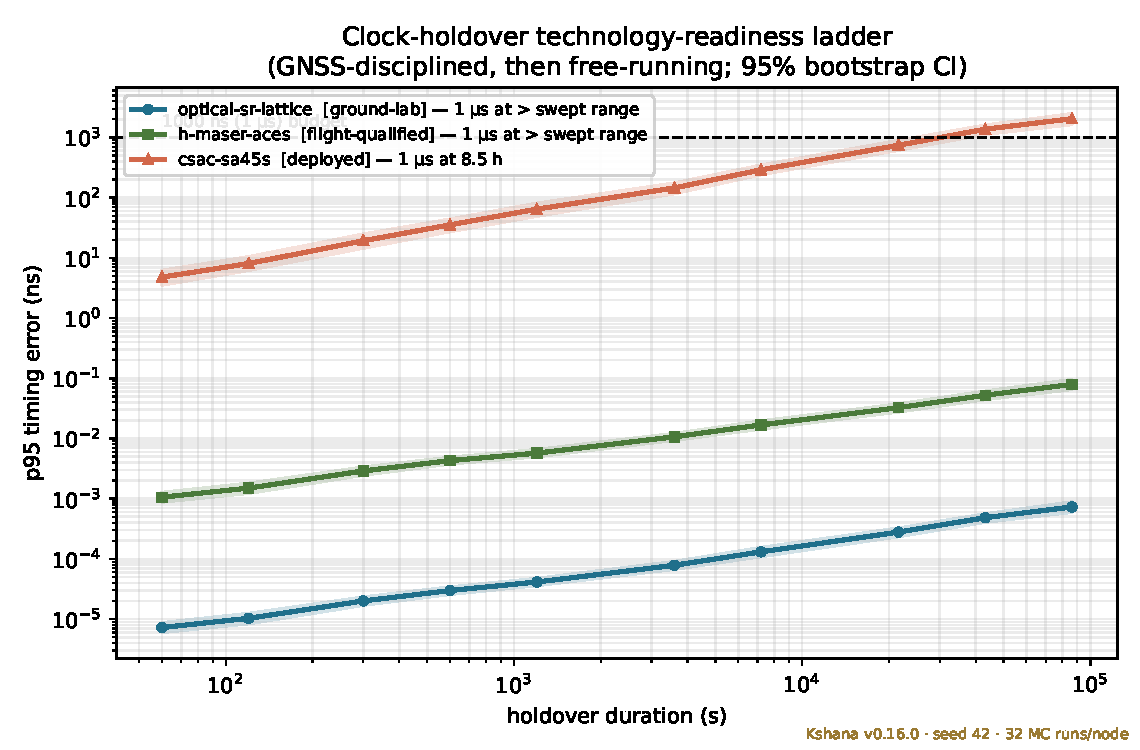
\includegraphics[width=0.8\linewidth]{clock.pdf}
  \caption{Clock holdover ladder. 95th-percentile timing error against a
  \SI{1}{\micro\second} budget as a function of holdover duration, for a
  ground-laboratory strontium optical-lattice clock (\citealp{origlia2015}), a
  flight-qualified ACES/PHARAO-class hydrogen maser, and a deployed chip-scale
  atomic clock. Each point is a 32-seed ensemble with a 95\% bootstrap interval and
  carries an inline technology-readiness tag. There is no winner-flip: the optical
  clock dominates stability, but its margin is a laboratory figure while the maser is
  the realistically flown option. The CSAC reaches the budget at $\approx$\SI{8.5}{\hour}.}
  \label{fig:clock}
\end{figure}

There is no crossover here, and reporting that honestly is the point. The
optical-lattice clock dominates the stability ranking at every holdover duration,
and both it and the maser hold the \SI{1}{\micro\second} budget essentially
indefinitely over the swept range: at \SI{24}{\hour} the optical clock's
95th-percentile holdover error is sub-nanosecond and the maser's is well under a
nanosecond, both three orders of magnitude inside budget. But the honest comparison
is the maturity-aware one. The optical clock's margin is a \emph{ground-laboratory}
figure; the maser is the option that has actually flown, and is therefore the
realistic on-orbit choice today. The deployed CSAC, by contrast, reaches the
\SI{1}{\micro\second} budget at $\approx$\SI{8.5}{\hour} of holdover --- a result
that matters operationally precisely because the CSAC is the rung that is already
fielded. The value of the ladder is that it refuses to compare a laboratory optical
clock against a deployed CSAC as if they were interchangeable, and instead pairs each
figure with the maturity tag that determines whether it is available to a mission.

\subsection{Time transfer: optical versus RF with a non-reciprocity budget}

The third lever compares optical inter-satellite time transfer against RF two-way
satellite time-and-frequency transfer (TWSTFT), and the methodological care is in
refusing the easy comparison. A jitter-only optical floor would report a figure that
no real two-way link achieves, because the limiting error in operational time
transfer is not jitter but \emph{non-reciprocity}: equipment-delay asymmetry between
the two terminals and path variation that does not cancel in the two-way difference.
We therefore model a non-reciprocal differential-delay budget for the optical link
\citep{giorgetta2013,deschenes2016} and adopt a conservative \SI{1}{\pico\second}
on-orbit optical target rather than the \SI{1}{\femto\second} laboratory floor, so
that the optical figure is charged with the same class of systematic that limits the
RF figure. Under this honest accounting the optical link reaches a range-equivalent
RMS of $\approx$\SI{0.29}{\milli\meter} (non-reciprocity included, a
\SI{1}{\pico\second} on-orbit projection target rather than a measured link budget)
against $\approx$\SI{341}{\milli\meter} for the RF link --- still a
three-order-of-magnitude advantage, but one obtained from a like-for-like budget
rather than from comparing an optical jitter floor against an RF link burdened with
systematics.

\subsection{What the map establishes}

Taken together, the three levers answer the question of \emph{when} quantum sensing
changes a PNT-resilience outcome, rather than asserting that it always does. The
inertial map shows a large but conditional advantage with a vibration-dependent
break-even that the classical sensor wins inside; the clock ladder shows a clear
stability ordering that is nonetheless governed by maturity, with no winner-flip to
overstate; and the time-transfer comparison shows a robust optical advantage only
once the optical figure is charged with the non-reciprocal systematics that limit
real links. Each figure in this section is reproducible from a committed scenario and
fixed seed using the commands listed in Appendix~A; the inertial and clock grids,
their break-even values, and their confidence intervals regenerate bit-for-bit from
the same machinery used for the validated packs.

\section{Validation}\label{sec:validation}

The trustworthiness of any comparison engine rests on whether its components
reproduce results that can be checked against an authority external to the
engine itself. Throughout this section we hold to a single discipline: every
number is compared against an external oracle (an independent reference
implementation, a published dataset, or an analytic closed form), and never
against Kshana's own output. We organise the evidence into three tiers ordered
by the strength of the external anchor, and we are explicit about what each tier
does and does not establish. Table~\ref{tab:validation} summarises the battery;
the prose below develops the caveats that the table can only flag.

\paragraph{Tier 1: bit-for-bit against an authoritative oracle.}
These checks reproduce an independent reference to within the numerical noise
floor, so agreement here speaks to correctness, not to a physical fit. The SGP4/SDP4 propagator reproduces all 666 verification states of
the AIAA 2006-6753 test set \citep{vallado2006} to a worst-case position error
of \SI{4.12}{\milli\metre} and velocity error of
\SI{1.85e-9}{\kilo\metre\per\second}. Against an independent Rust
implementation, the \code{sgp4} crate \citep{sgp4crate}, agreement is sub-micron
on the near-earth and resonant orbits and \SI{4.12}{\milli\metre} in the
worst case across all regimes; we therefore do not claim blanket sub-micron
agreement. The IAU~2000A nutation routine \code{eraNut00a} reproduces the SOFA
reference values $\Delta\psi = -0.96309\times10^{-5}$~rad and
$\Delta\epsilon = +0.40632\times10^{-4}$~rad to $10^{-13}$~rad
\citep{iausofa}. The frame transformations match the Vallado worked examples
\citep{vallado2006,iausofa} to \SI{0.1}{\milli\metre} (TEME$\rightarrow$PEF),
\SI{0.6}{\milli\metre} (TEME$\rightarrow$ITRF), and \SI{4}{\milli\metre} for the
full CIO-based GCRS$\rightarrow$ITRS chain. The Allan-deviation estimator
reproduces the Stable32/NBS14 reference series \citep{stable32,riley2008nist} to
a relative error of $10^{-4}$. The dilution-of-precision computation matches the
closed-form regular-tetrahedron geometry \citep{misra2010,kaplan2017} exactly:
$\mathrm{GDOP}=\sqrt{10}/2=1.5811$, $\mathrm{PDOP}=1.5$, $\mathrm{TDOP}=0.5$.
The inertial error model reproduces the velocity- and angle-random-walk
coefficients of the NaveGo 3DM-GX3-35 reference profiles
\citep{gonzalez2017navego} to within $5\%$. Finally, the two-body propagator
agrees with an independent universal-variable Kepler solver to sub-metre over
\SI{24}{\hour}, conserving energy and angular momentum to $\sim10^{-9}$
(relative). Tier~1 is the strongest evidence in the paper: each row is an
independent oracle, and the residuals are numerical, not physical.

\paragraph{Tier 2: post-fit residual against real agency truth.}
Tier~2 reports how closely Kshana's dynamics can be made to track precise
ephemerides published by space agencies. This is a \emph{force-model validation
by ephemeris fitting}, not orbit determination: there is no measurement
processing, and the residual is the post-fit overlap of a fitted trajectory
against the agency product. The arc length, gravity-field degree and order, and
empirical-acceleration tier are stated inline for every entry because they
determine what the residual means. Our headline is the Galileo MEO full-arc
result: a \SI{0.61}{\metre} post-fit residual over a \SI{24}{\hour} arc with a
degree/order-70 gravity field and no empirical accelerations, the configuration
that most directly exercises force-model fidelity. On the shorter \SI{8}{\hour} CI
arc the pure-force fit is \SI{0.13}{\metre}, and the reduced-dynamic tier, in
which per-revolution empirical accelerations are estimated alongside the
trajectory, lowers it further to \SI{0.07}{\metre}; the same reduced-dynamic tier
yields \SI{0.10}{\metre} for the Swarm-A LEO arc
\citep{montenbruck2000,petit2010iers}. We emphasise that these reduced-dynamic
numbers \emph{bound} force-model accuracy rather than measure it: the estimated
empirical accelerations absorb mismodelled dynamics, so a small reduced-dynamic
residual is an upper bound on, not a measurement of, the underlying force-model
error. They are reported as clearly-labelled secondary lines, never as the
headline.

The lunar case is stated as honestly as the favourable ones. The LRO arc yields
a \SI{6.6}{\metre} reduced-dynamic residual, which is \emph{above} our
\SI{5}{\metre} target \citep{lemoine2013grail,giorgini1996horizons}; we report
the miss rather than tuning it away. As a controlled cross-validation, we swap
the analytic kernel-free ephemeris for a DE440 realisation via ANISE: the LRO
reduced-dynamic residual is unchanged at the centimetre level
($6.65\rightarrow\SI{6.67}{\metre}$). This reproduces an established
result, that a carefully constructed analytic stack matches a DE-grade
ephemeris realisation for this class of arc \citep{bertone2021grail,li2023leopod};
it is not a discovery, and it is scoped to the LRO arc only. We credit
\code{nyx}/ANISE \citep{nyxanise} as the DE-grade oracle against which the swap
is checked, not as a rival the engine outperforms.

\paragraph{Tier 3: parameter-level characterisation.}
The multi-layer spoofing detector (per-epoch RAIM parity, automatic-gain-control
monitoring, signal-quality monitoring, and a fusion stage) is characterised
against the \emph{published scenario parameters} of the TEXBAT corpus
\citep{humphreys2012texbat}: the hand-coded inputs and expected outputs are
derived from the documented scenario descriptions. The detector ingests no
TEXBAT samples; raw-IQ ingestion is future work. We are explicit that this is
not external validation. Tier~3 establishes that the detection logic responds as
expected to parameter regimes drawn from a real corpus, but until raw IQ is
processed it cannot be called a validation against TEXBAT, and Table~\ref{tab:validation}
labels it accordingly.

\paragraph{Reading the table.}
The status vocabulary mirrors the methodology of Section~\ref{sec:method}.
Tier~1 rows are \emph{validated} against an external oracle to the numerical
floor. Tier~2 rows are \emph{validated by ephemeris fitting}: a genuine
external anchor (the agency product), but a fit, with the empirical-tier caveat
made explicit. Tier~3 is \emph{characterised, not validated}. None of these
rows involves a quantum figure of merit: the quantum-sensor performance models
are projections from cited device coefficients, treated in
Section~\ref{sec:crossover} and never entered into this external-validation
battery.

\begin{table}[t]
\centering
\small
\setlength{\tabcolsep}{5pt}
\renewcommand{\arraystretch}{1.25}
\caption{External-validation battery, tiered by the strength of the external
anchor. Every result is compared against an oracle independent of the engine.
Tier~1 reproduces an authoritative reference to the numerical floor; Tier~2
reports post-fit residuals against agency precise ephemerides (a force-model fit
by ephemeris fitting, with arc length, gravity degree/order, and
empirical-acceleration tier stated inline); Tier~3 is parameter-level
characterisation, not external validation. Reduced-dynamic residuals bound, and
do not measure, force-model accuracy.}
\label{tab:validation}
\begin{tabular}{@{}p{0.255\linewidth} p{0.215\linewidth} p{0.295\linewidth} p{0.155\linewidth}@{}}
\toprule
\textbf{Check} & \textbf{Oracle} & \textbf{Result} & \textbf{Status} \\
\midrule
\multicolumn{4}{@{}l}{\textit{Tier 1: bit-for-bit vs.\ authoritative oracle}}\\
\addlinespace[2pt]
SGP4/SDP4, 666 states &
AIAA 2006-6753 \citep{vallado2006} &
\SI{4.12}{\milli\metre} pos., \SI{1.85e-9}{\kilo\metre\per\second} vel.\ (worst case) &
Validated \\
SGP4 head-to-head &
\code{sgp4} crate \citep{sgp4crate} &
sub-\si{\micro\metre} near-earth/resonant; \SI{4.12}{\milli\metre} worst case all regimes &
Validated \\
Nutation \code{eraNut00a} &
SOFA/ERFA \citep{iausofa} &
$\Delta\psi=-0.96309\!\times\!10^{-5}$, $\Delta\epsilon=+0.40632\!\times\!10^{-4}$~rad to $10^{-13}$ &
Validated \\
Frame transforms &
Vallado \citep{vallado2006,iausofa} &
TEME$\to$PEF \SI{0.1}{\milli\metre}; TEME$\to$ITRF \SI{0.6}{\milli\metre}; GCRS$\to$ITRS \SI{4}{\milli\metre} &
Validated \\
Allan deviation &
Stable32/NBS14 \citep{stable32,riley2008nist} &
relative error $10^{-4}$ &
Validated \\
GDOP/PDOP/TDOP &
closed form \citep{misra2010,kaplan2017} &
$\sqrt{10}/2=1.5811$; $1.5$; $0.5$ (exact) &
Validated \\
Inertial VRW/ARW &
NaveGo 3DM-GX3-35 \citep{gonzalez2017navego} &
within $5\%$ &
Validated \\
Two-body propagation &
universal-variable Kepler &
sub-metre / \SI{24}{\hour}; energy + ang.\ mom.\ to $\sim10^{-9}$ &
Validated \\
\addlinespace[3pt]
\multicolumn{4}{@{}l}{\textit{Tier 2: post-fit residual vs.\ agency truth (force-model fit by ephemeris fitting)}}\\
\addlinespace[2pt]
Galileo MEO (headline) &
agency precise eph.\ \citep{montenbruck2000,petit2010iers} &
\SI{0.61}{\metre}, \SI{24}{\hour} arc, d/o~70, force-only &
Validated (fit) \\
Galileo MEO (\SI{8}{\hour}, reduced-dynamic) &
agency precise eph.\ \citep{montenbruck2000,petit2010iers} &
\SI{0.07}{\metre} (\SI{0.13}{\metre} pure-force); empirical-accel tier (bounds, not measures) &
Validated (fit) \\
Swarm-A LEO (reduced-dynamic) &
agency precise eph.\ \citep{montenbruck2000,petit2010iers} &
\SI{0.10}{\metre}; empirical-accel tier (bounds, not measures) &
Validated (fit) \\
LRO lunar &
GRGM \citep{lemoine2013grail,giorgini1996horizons} &
\SI{6.6}{\metre} reduced-dynamic, \emph{above} \SI{5}{\metre} target (honest miss) &
Validated (fit) \\
LRO DE440/ANISE swap &
\code{nyx}/ANISE \citep{nyxanise,bertone2021grail,li2023leopod} &
residual unchanged $6.65\!\to\!\SI{6.67}{\metre}$; reproduces known result, LRO-scoped &
Validated (fit) \\
\addlinespace[3pt]
\multicolumn{4}{@{}l}{\textit{Tier 3: parameter-level characterisation (not external validation)}}\\
\addlinespace[2pt]
Spoofing detector (RAIM + AGC + SQM + fusion) &
TEXBAT scenario \emph{parameters} \citep{humphreys2012texbat} &
responds as expected to documented parameter regimes; raw-IQ ingestion is future work &
Characterised, not validated \\
\bottomrule
\end{tabular}
\end{table}

\section{Limitations and threats to validity}\label{sec:limitations}

The following disclosures form part of the honesty contract that the methodology
in Section~\ref{sec:method} demands. Every figure of merit is reported alongside the
strength of the evidence that backs it, and a result that is a model projection or a
force-model fit is never dressed as a measurement. The same discipline applies to the
boundaries of the engine itself.

\begin{itemize}

  \item \textbf{Quantum-sensor figures are projections, not measurements.}
  Every cold-atom inertial, optical-lattice clock, and optical time-transfer number
  in this paper (including the crossover and break-even results of
  Section~\ref{sec:crossover}) is a performance-model projection computed by
  deterministic arithmetic on coefficients drawn from the cited device literature
  \citep{templier2022,origlia2015,giorgetta2013,deschenes2016}, not data from
  operating hardware. We carry an inline maturity tag (flight-qualified /
  ground-lab / projection-floor) on every quantum point for exactly this reason
  (Figure~\ref{fig:clock}). For time transfer we keep the comparison like-for-like:
  the reported optical figure is charged with a conservative non-reciprocal
  differential-delay budget (a \SI{1}{\pico\second} on-orbit target, not the
  \SI{1}{\femto\second} laboratory floor), so it carries the same class of systematic
  that limits the RF figure (Section~\ref{sec:crossover}). A jitter-only optical floor
  would exclude that non-reciprocity and overstate the optical advantage; we do not
  report it.

  \item \textbf{The agency-orbit work is a force-model fit, not orbit
  determination.} The residuals against agency precise ephemerides
  (Table~\ref{tab:validation}) are obtained by \emph{force-model validation by ephemeris
  fitting} (propagation-overlap consistency against an external truth product), not by
  processing observations. The headline is the full-arc Galileo result,
  \SI{0.61}{\metre} over \SI{24}{\hour} at gravity-field degree/order~70. The
  reduced-dynamic tier on the \SI{8}{\hour} arc (Galileo \SI{0.07}{\metre} from a
  \SI{0.13}{\metre} pure-force fit, Swarm \SI{0.10}{\metre}) admits
  empirical accelerations that absorb mismodelled dynamics; these numbers
  \emph{bound}, and do not \emph{measure}, force-model accuracy, and we label them
  reduced-dynamic wherever they appear. The fits are single-satellite, single-day
  arcs; they are not a statistical population over regimes.

  \item \textbf{LRO is above the target.} The LRO reduced-dynamic
  residual is \SI{6.6}{\metre}, above our \SI{5}{\metre} target. Swapping the default
  ephemeris for a DE440/ANISE realisation leaves it essentially unchanged
  (\SI{6.65}{\metre} $\rightarrow$ \SI{6.67}{\metre}). We present this as a
  controlled reproduction of a known result \citep{bertone2021grail,li2023leopod},
  scoped to the LRO arc only and not a discovery, and we credit \texttt{nyx}/ANISE
  \citep{nyxanise} as the DE-grade oracle, not a rival the engine outperforms.

  \item \textbf{The spoofing detector does not ingest raw IQ.} It is characterised
  against published TEXBAT \emph{parameters} \citep{humphreys2012texbat} using
  hand-coded inputs and expected outputs; it does not read the TEXBAT recordings.
  Consequently we report no receiver-operating-characteristic curve and no
  $P_d$/$P_{fa}$ operating point. Raw-IQ ingestion is future work, and the detector
  sits in the not-externally-validated tier of Table~\ref{tab:validation}.

  \item \textbf{Single-point positioning is code-only, not carrier-phase
  PPP/RTK.} The engine spans the measurement-to-position gap with a code
  single-point-positioning solver: it ingests real RINEX pseudoranges and
  broadcast ephemeris and returns a receiver position by iterated weighted
  least squares (Sagnac and broadcast satellite-clock corrections, the
  dual-frequency L1/L2 ionosphere-free combination, and a Saastamoinen/Niell
  troposphere), recovering the surveyed coordinate of IGS station ABMF to
  \SI{5.7}{\metre} 3-D RMS (\SI{1.1}{\metre} horizontal). This is metre-level
  \emph{code} positioning, not carrier-phase precise positioning: there is no
  ambiguity resolution, carrier smoothing, or inter-epoch filter, so the
  centimetre-grade PPP/RTK domain remains that of dedicated tools such as RTKLIB
  \citep{takasu2009} (Table~\ref{tab:intersection}). The paper's central
  contribution is the resilience-comparison methodology of
  Section~\ref{sec:method}, not a competition on positioning accuracy, and this
  single-station code fix is a boundary capability rather than a member of the
  external-validation battery of Table~\ref{tab:validation}.

  \item \textbf{Modelling-fidelity defaults are deliberately modest.} The inertial
  mechanisation is 1-DOF, not a full 3-axis strapdown solution \citep{groves2013};
  atmospheric drag uses a static exponential density profile rather than NRLMSISE-00;
  solar radiation pressure is a cannonball model; relativity is Schwarzschild-only;
  and the default ephemerides are low-precision. Each is adequate for the
  comparison-under-uncertainty role and is overridden by the higher-fidelity paths
  only where a validation result requires it.

  \item \textbf{Time representation is single-\texttt{f64} Julian date.} A single
  double-precision Julian date gives roughly \SI{50}{\micro\second} resolution near
  the present epoch, which is immaterial for the resilience figures of merit reported
  here but would matter for sub-microsecond timing applications.

  \item \textbf{In-browser execution is a deployment property, not a capability.}
  Running the integrated stack zero-install in WASM lowers the barrier to
  reproduction; it does not extend what the engine computes. In-browser SGP4 is not
  itself new \citep{satellitejs}; the delta is a single engine running the full
  integrated stack with no installation.

\end{itemize}

\noindent Collectively these bounds define what the engine establishes: a
reproducible, falsifiable comparison framework with an external-validation battery
behind it. They equally define what it does not: it is not a measurement
campaign, not an orbit-determination system, and not a fielded quantum-sensing
result.

\section{Discussion and conclusion}\label{sec:discussion}

The methodology of Section~\ref{sec:method}, together with the crossover map of
Section~\ref{sec:crossover}, is intended to make one specific question answerable in
a neutral, reproducible way: \emph{what resilience does a given sensor architecture
buy, and over what operating envelope?} Rather than asserting a verdict, Kshana
\citep{baweja2026kshana} fixes a scenario, a seed, and an engine version, routes the
quantum and classical candidates through a single code path, and labels every
figure-of-merit as externally validated or merely modelled. The output of that
discipline is not a marketing number but an envelope: a region of the operating space
in which one architecture dominates, a region in which it does not, and a break-even
boundary between them carried with a $95\%$ confidence band.

This reframing matters because the comparison it supports is different from the one the
literature usually runs. The question \emph{``is quantum sensing better?''} is already
well populated by device papers and surveys
\citep{templier2022,coldatomnavreview2022,quantumpntreview2026}; it is answered
affirmatively on isolated axes and, on its own, settles little for a system designer.
The crossover map asks instead \emph{``where does the quantum lever change the
outcome?''}, and answers it openly, with the uncertainty made explicit rather than
hidden. The inertial study locates that boundary as a vibration tolerance that grows
with outage duration --- the break-even platform-vibration PSD rises from the order of
$10^{-5}$ at a $30$~s outage to the order of $10^{-4}$~(m/s$^2$)$^2$/Hz near a
$1800$~s outage --- so the cold-atom advantage is real for long, quiet holdovers and
erodes under aggressive platform vibration, exactly where a TRL-honest answer should
place it. The clock study is starker still: the deployed chip-scale reference crosses a
$1\,\mu$s timing budget at roughly $3.0\times10^{4}$~s ($\sim$8.5~h) of holdover, while
the ground-lab optical-lattice and flight-qualified maser curves stay below that budget
across the full $24$~h sweep. These are performance-model projections from cited device
coefficients, not measurements, and they are TRL-tagged as such; the contribution is the
reproducible map and its break-even contour, not any single point on it.

Interoperability is what turns this from a closed demonstrator into an on-ramp. Because
the engine reads and writes the standard exchange formats (RINEX, SP3, CCSDS OEM/OMM),
a crossover study or a propagated state can move into established pipelines --- RTKLIB
\citep{takasu2009}, GMAT \citep{nasa_gmat}, Orekit \citep{orekit} --- rather than
living only inside Kshana. The single integrated stack runs natively, from Python, and
in the browser via WebAssembly; in-browser SGP4 is not itself new
\citep{satellitejs,sgp4crate}, and the delta is only that one engine runs the full
integrated stack with zero install, lowering the cost of reproducing a result to opening
a page.

Several limitations defined in Section~\ref{sec:limitations} double as the natural work
ahead. The PVT path is scenario-driven rather than fed by real observations; ingesting
real GNSS observations to close a measurement-level loop is the most consequential next
step. The spoofing detector is characterised against published TEXBAT
\citep{humphreys2012texbat} parameters, not raw IQ; ingesting raw IQ and reporting a
detection ROC would move it from the not-externally-validated tier into a measured one.
The force-model validation by ephemeris fitting reported in
Section~\ref{sec:validation} is single-arc and single-satellite; extending it to
multi-satellite, multi-day fits would tighten the residual envelope and test the static
drag, cannonball-SRP, and Schwarzschild defaults under more diverse dynamics. Finally,
the crossover map presently sweeps published-parameter envelopes one lever at a time;
propagating the full coefficient uncertainty jointly --- and adding same-TRL pairings
across all three levers --- would turn today's three studies into a single crossover
atlas of resilient PNT.

What we offer, then, is less a claim of superiority than a way of arguing about it
honestly. The agency-orbit work is a force-model validation by ephemeris fitting, not
orbit determination; the headline full-arc Galileo residual is $0.61$~m at degree and
order $70$, with the $0.13$~m and $0.10$~m reduced-dynamic figures stated as
empirical-acceleration-tier bounds rather than measures of force-model accuracy; the
LRO residual is $6.6$~m, above the $5$~m target, reported as such and reproduced as a
known result \citep{bertone2021grail,li2023leopod} against a DE-grade ANISE oracle
\citep{nyxanise} that we credit rather than claim to beat; and every quantum figure is a
projection, every spoofing claim a parameter-level characterisation. To our knowledge no
open tool runs this full integrated PNT-resilience stack with these honesty controls
attached. That stance --- validated-or-not-modelled stated per figure-of-merit, the
quantum-versus-classical axis swapped through one neutral code path, and every headline
number traceable to a committed scenario, seed, and test --- is the differentiator we
mean to defend, consistent with the reproducibility tradition this work builds on
\citep{fernandezprades2018reproducibility,nasastd7009}.

\section*{Data and code availability}

Kshana is open-source software released under the Apache-2.0 licence
\citep{baweja2026kshana}. Each tagged release is archived on Zenodo
(DOI~\href{https://doi.org/10.5281/zenodo.20528627}{10.5281/zenodo.20528627}),
which provides a citable, immutable snapshot of the exact source used to produce
the results in this paper. The engine ships as native binaries, as a PyPI package,
and as a zero-install WebAssembly playground that runs the full integrated stack
in the browser.

The crossover study of Section~\ref{sec:crossover}, every figure, and every
headline number in this paper regenerate from a fixed scenario plus seed. The exact
commands are given in Appendix~\ref{app:repro}; running them against the archived
release reproduces the reported values bit-for-bit where the underlying check is
deterministic.


\bibliographystyle{plainnat}
\bibliography{../paper,refs-extra}

\appendix
\section{Reproducibility}\label{app:repro}

Every result in this paper is regenerable from a committed scenario, a fixed
random seed, and a pinned engine version (\texttt{0.17.0}); no figure or number
depends on hidden state. The commands below regenerate the new crossover result
(\S\ref{sec:crossover}) and its figures, and re-run the external-validation
oracles (\S\ref{sec:validation}).

The crossover study writes the inertial and clock sweep results
(\texttt{inertial.json}, \texttt{clock.json}) with seed \texttt{42} fixed, and
the two render scripts produce Figures~\ref{fig:inertial} and~\ref{fig:clock}
directly from that JSON:

\begin{verbatim}
# crossover study JSON (inertial + clock), fixed seed 42
cargo run --release --bin crossover_study -- paper/crossover
# figures
python3 paper/crossover/render_inertial.py paper/crossover/inertial.json
python3 paper/crossover/render_clock.py     paper/crossover/clock.json
# time-transfer lever (optical vs RF), seed 42
cargo run --release -- scenarios/timetransfer.toml
# validation oracles (examples)
cargo test --test sgp4_verification
cargo test --test frame_reference_vectors
cargo test --test agency_galileo
\end{verbatim}

The \code{agency\_galileo} test reproduces the \SI{8}{\hour} continuous-integration
fixture (pure-force \SI{0.13}{\metre}, reduced-dynamic \SI{0.07}{\metre} at
degree/order~12, which is gravity-converged); the \SI{0.61}{\metre}, \SI{24}{\hour},
degree/order-70 \emph{headline} is produced by the \code{galileo\_full\_arc\_dispatch}
job (an \code{\#[ignore]}d test that fetches the full-day agency ephemeris;
\code{KSHANA\_GALILEO\_DEGREE} defaults to 70).

The validation tests are self-checking: each derives its expected values from an
external reference -- the AIAA/Vallado verification set for SGP4, SOFA/ERFA
reference vectors for the frame transformations, and agency precise ephemerides
for the force-model fit by ephemeris fitting -- rather than from the engine
itself. Expected values are hand-entered or read from the cited dataset, so a
passing test cross-validates Kshana against an independent oracle. The committed
JSON artifacts (\texttt{inertial.json}, \texttt{clock.json}) carry the engine
version and the full parameter envelope as metadata, so a reader can confirm that
the figures in this paper correspond bit-for-bit to a re-run on the same engine
version and seed. Full build instructions and the Zenodo archive are linked from
the repository \citep{baweja2026kshana}.


\end{document}
